\documentclass[12pt]{article}
\usepackage[utf8]{inputenc}
\usepackage[brazil]{babel}
\usepackage{amsmath, amssymb}
\usepackage{graphicx}
\usepackage{listings}
\usepackage{color}
\usepackage{caption}
\usepackage{subcaption}
\usepackage[hidelinks]{hyperref}
\usepackage{geometry}
\geometry{margin=2.5cm}
\usepackage{algorithm}
\usepackage{algpseudocode}
\usepackage{float}
\usepackage{booktabs}
\usepackage{tabularx}


\title{Análise de Grafos de Coocorrência de Termos em Textos Científicos}
\author{Lincoln Gondin; Gustavo Henrique}
\date{Junho 2025}

\begin{document}

\maketitle

\tableofcontents
\newpage

\section{Descrição da Extração de Termos}

Para a base de textos científicos foi utilizado os resumos dos textos encontrados no site \textit{arxiv.org}. O arXiv é um serviço de distribuição gratuita e aberta para mais de 2,4 milhões de artigos científicos, em uma série de campos de estudo.

Para a extração foi feito um script em Python para o \textit{scraping} dos resumos de vários textos científicos em todas as categorias disponíveis no site, sendo elas: Ciência da Computação, Economia, Engenharia Elétrica e Ciência de Sistemas, Matemática, Física, Biologia Quantitativa, Finança Quantitativa e Estatística.

Foram extraídos 1466 resumos dessas diferentes categorias e salvos em arquivos de texto separados para posterior processamento.

\section{Construção do Grafo de Coocorrência}

O grafo foi construido seguindo uma implementação direta do pseucodigo que podemos visualizar abaixo. Cada termo da base de texto se traduziu em um vertice e se os termos coocorrem na mesma janela ao menos uma vez uma aresta unica é criada entre eles. Foi utilizado grafos não direcionados para as análises.

\begin{algorithm}[H]
\caption{Geração do Grafo de Coocorrência}
\begin{algorithmic}[1]
\Function{GerarGrafoCoocorrencia}{representacao, textos, textosOriginais, $n$, $w$}
    \State $Voc \gets$ \Call{ColetarNTermosMaisFrequentes}{$n$, textos}
    \State $mapa\_indices \gets$ mapa de cada termo em $Voc$ para seu índice
    \If{representacao é ``lista''}
        \State $grafo \gets$ \Call{GrafoLista}{$Voc$}
    \Else
        \State $grafo \gets$ \Call{GrafoMatriz}{$Voc$}
    \EndIf

    \For{cada texto $T$ em $textosOriginais$}
        \For{$i \gets 0$ até $|T| - w$}
            \State $janela \gets T[i:i+w]$
            \State $termos \gets$ termos da janela que estão em $mapa\_indices$
            \State $pares \gets$ todas as combinações únicas de dois termos em $termos$
            \For{cada par $(t_a, t_b)$ em $pares$}
                \State $u \gets mapa\_indices[t_a]$
                \State $v \gets mapa\_indices[t_b]$
                \If{não \Call{grafo.arestaExiste}{$u, v$}}
                    \State \Call{grafo.adicionarAresta}{$u, v$}
                \EndIf
            \EndFor
        \EndFor
    \EndFor
    \State \Return $grafo$
\EndFunction
\end{algorithmic}
\end{algorithm}



\section{Representações de Grafo}

Foi utilizada uma abordagem OOP para a criação das duas representações dos grafos, dessa maneira ambas possuiam a mesma interface de interação.

Por conta dessa escolha tecnica não foi necessario, por exemplo criar duas funções diferentes dos algoritmos de detecção de componentes conexas. É possivel visualizar na figura abaixo a classe base que a representação em lista e em matriz herdam. Cada representação terá sua própria implementação para cada função.

\begin{figure}[H]
    \centering
    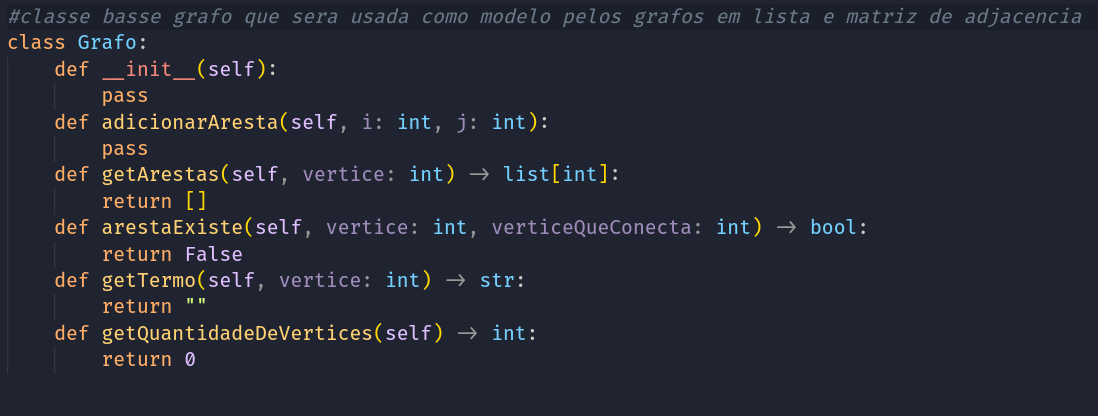
\includegraphics[width=1\textwidth]{classBase.png}
    \caption{Classe Grafo base.}
\end{figure}

\subsection{Lista de Adjacência}
A representação em lista foi feita como se é esperado; cada vertice armazena uma lista de todos os seus vertices vizinhos, representado-os por inteiros, para a consulta do termo ao qual o vertice se refere foi utilizado uma lista externa onde o i-esimo elemento representa o i-esimo termo extraido da base de texto, o mesmo foi feito na representação em matriz. 

\begin{figure}[H]
    \centering
    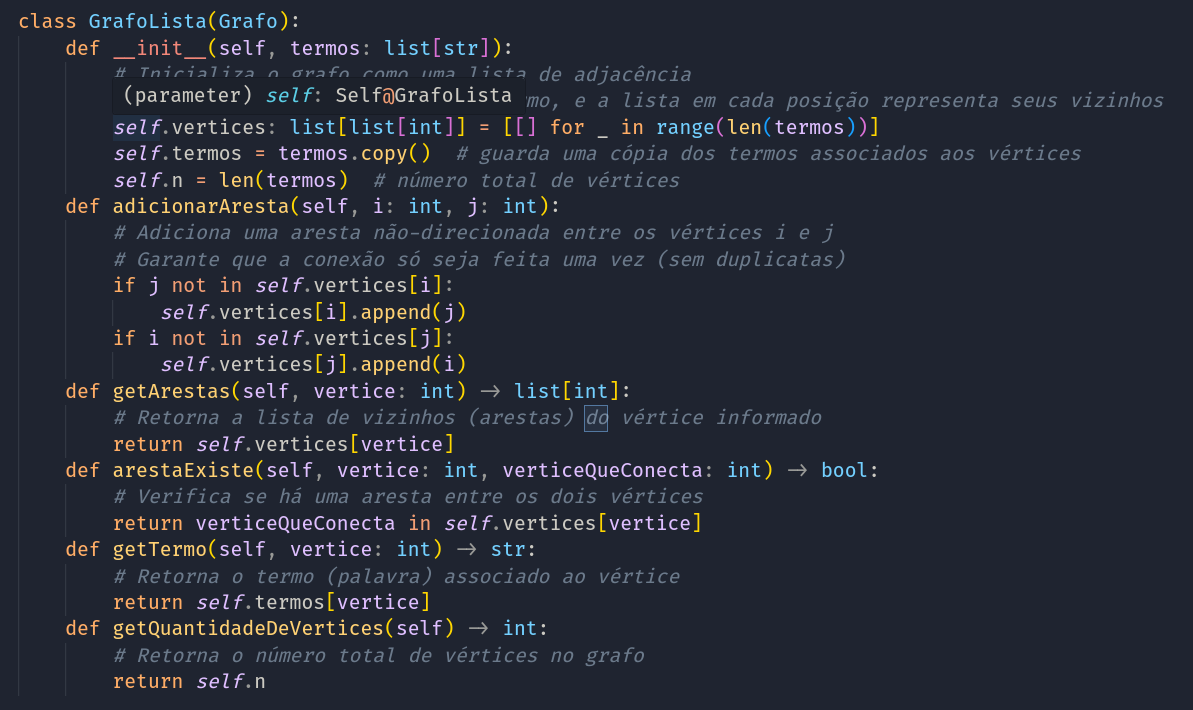
\includegraphics[width=1\textwidth]{grafoLista.png}
    \caption{Implementação do grafo usando lista de adjacência.}
\end{figure}

\subsection{Matriz de Adjacência}
Na representação em matriz foi utilizado uma lista bidimensional n por n, onde o elemento Aij é 1 caso haja uma aresta de i para j.

\begin{figure}[H]
    \centering
    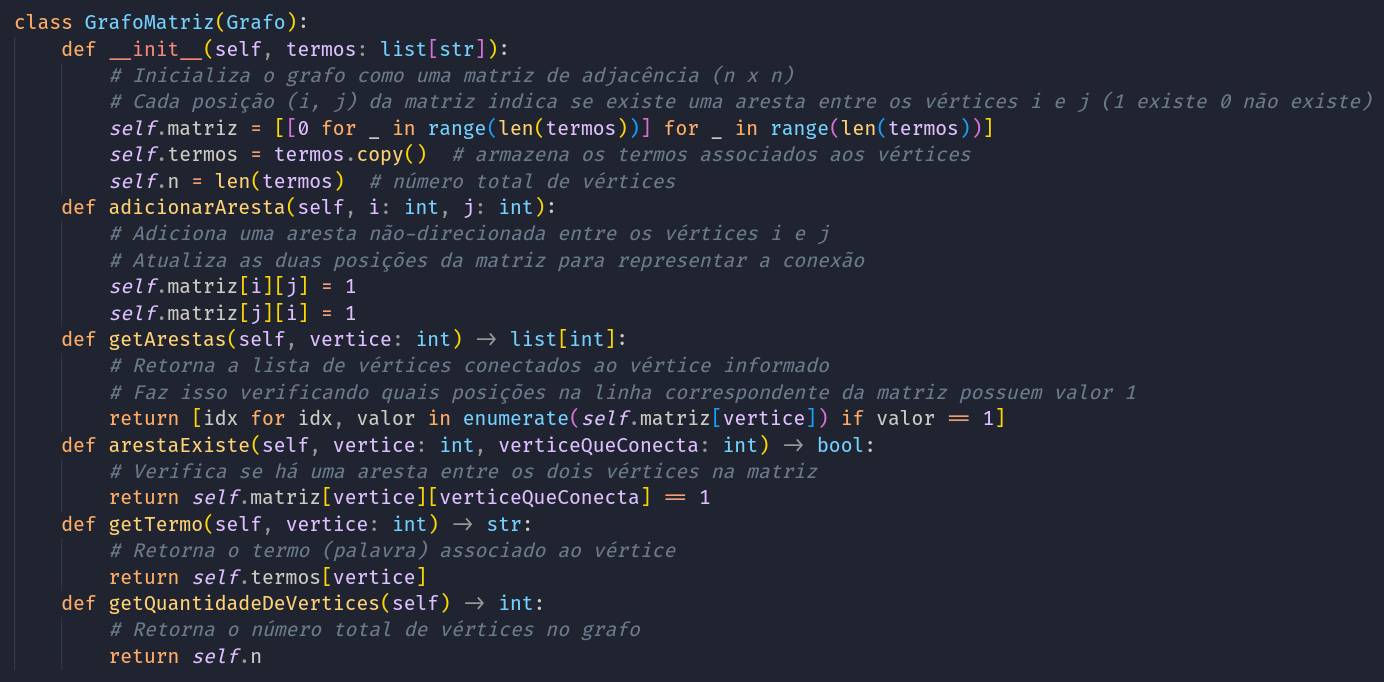
\includegraphics[width=1\textwidth]{grafoMatriz.png}
    \caption{Implementação do grafo usando matriz de adjacência.}
\end{figure}

\section{Algoritmos para Detecção de Componentes Conectados}

\subsection{Força Bruta (Grafo Não Direcionado)}

O algoritmo de força bruta para detecção de componentes conexas em grafos não direcionados utiliza uma busca em profundidade (DFS) iniciada a partir de cada vértice não visitado. A cada nova DFS, é identificada uma nova componente conexa, agrupando todos os vértices acessíveis a partir daquele ponto inicial. O processo se repete até que todos os vértices tenham sido visitados. É uma abordagem simples e eficaz para grafos não direcionados e densos.

\begin{algorithm}[H]
\caption{Algoritmo de Força Bruta para Componentes Conexas}
\begin{algorithmic}[1]
\Function{ForcaBrutaComponentes}{grafo}
    \State visitado $\gets$ vetor de tamanho $n$ inicializado com \textbf{FALSO}
    \State componentes $\gets$ lista vazia
    \For{$v \gets 0$ até $n - 1$}
        \If{não visitado[$v$]}
            \State componente $\gets$ lista vazia
            \State \Call{DFS}{$v$, componente}
            \State Adicionar componente à lista componentes
        \EndIf
    \EndFor
    \State \Return componentes
\EndFunction

\Function{DFS}{$v$, componente}
    \State visitado[$v$] $\gets$ \textbf{VERDADEIRO}
    \State Adicionar $v$ à lista componente
    \For{cada vizinho em \Call{grafo.getArestas}{$v$}}
        \If{não visitado[vizinho]}
            \State \Call{DFS}{vizinho, componente}
        \EndIf
    \EndFor
\EndFunction
\end{algorithmic}
\end{algorithm}

\subsection{Algoritmo Adaptado de Tarjan (Grafo Não Direcionado)}

A versão original do algoritmo de Tarjan foi desenvolvida para encontrar componentes fortemente conexas em grafos direcionados. No entanto, ao lidar com grafos não direcionados, o uso direto da versão clássica de Tarjan pode causar problemas, como a identificação errada de conexões ou loops desnecessários. Por isso, uma adaptação foi realizada: ao invés da abordagem recursiva baseada em índices e low-link, utiliza-se uma DFS iterativa com pilha, que mantém o rastreamento de vértices visitados para formar as componentes conexas de forma eficiente e compatível com grafos não direcionados.

\begin{algorithm}[H]
\caption{Versão Iterativa do Algoritmo de Tarjan para Componentes Conexas}
\begin{algorithmic}[1]
\Function{TarjanAdaptado}{grafo}
    \State visitado $\gets$ vetor de tamanho $n$ inicializado com \textbf{FALSO}
    \State componentes $\gets$ lista vazia
    \For{$v \gets 0$ até $n - 1$}
        \If{não visitado[$v$]}
            \State componente $\gets$ \Call{DFS}{$v$}
            \State Adicionar componente à lista componentes
        \EndIf
    \EndFor
    \State \Return componentes
\EndFunction

\Function{DFS}{$v_{\text{inicial}}$}
    \State pilha $\gets$ lista contendo $v_{\text{inicial}}$
    \State componente $\gets$ lista vazia
    \State visitado[$v_{\text{inicial}}$] $\gets$ \textbf{VERDADEIRO}
    \While{pilha não está vazia}
        \State $v \gets$ pilha.pop()
        \State Adicionar $v$ à lista componente
        \For{cada vizinho em \Call{grafo.getArestas}{$v$}}
            \If{não visitado[vizinho]}
                \State visitado[vizinho] $\gets$ \textbf{VERDADEIRO}
                \State pilha.push(vizinho)
            \EndIf
        \EndFor
    \EndWhile
    \State \Return componente
\EndFunction
\end{algorithmic}
\end{algorithm}



\section{Procedimento de Medição de Tempo}

Para avaliar o desempenho dos algoritmos de detecção de componentes conexas implementados neste trabalho, foi desenvolvido um sistema de medição de tempo de execução. O objetivo é comparar a eficiência das abordagens (Força Bruta e Tarjan adaptado), bem como o impacto da representação do grafo (lista ou matriz de adjacência) sobre o tempo de execução.

\subsection{Função de Medição de Tempo Individual}

A função \texttt{medir\_tempo\_algoritmo} executa um determinado algoritmo sobre um grafo, repetidas vezes, e retorna o tempo médio de execução em milissegundos. Ela recebe como parâmetros:

\begin{itemize}
    \item \textbf{nome\_algoritmo}: nome do algoritmo a ser testado (apenas para fins de exibição);
    \item \textbf{representacao}: tipo de estrutura utilizada (lista ou matriz);
    \item \textbf{funcao}: referência à função do algoritmo que será executado;
    \item \textbf{grafo}: o grafo sobre o qual o algoritmo será executado;
    \item \textbf{quantidade\_execucoes}: número de vezes que a função será chamada para cálculo da média.
\end{itemize}

O tempo total é medido com a função \texttt{time.perf\_counter()}, que fornece alta resolução para medições de desempenho.

\subsection{Função de Medição Global}

A função \texttt{medirDesempenho} organiza os testes para três tamanhos diferentes de grafo, com 500, 1000 e 2000 termos mais frequentes extraídos dos textos. Para cada tamanho, são criadas representações dos grafos em lista e matriz de adjacência. Em seguida, são realizados testes para os dois algoritmos (Força Bruta e Tarjan adaptado) sobre ambas as representações.

\begin{itemize}
    \item Para cada combinação algoritmo/representação, o tempo médio de execução é calculado;
    \item Os resultados são armazenados em um dicionário para posterior geração de gráficos comparativos;
    \item A quantidade de execuções padrão utilizada foi de 1.000.000 repetições por teste.
\end{itemize}

Este processo garante que as variações causadas por pequenas flutuações de desempenho da máquina não interfiram significativamente nos resultados.

\subsection{Pseudocódigo das Funções de Medição}

\begin{algorithm}[H]
\caption{Função medir\_tempo\_algoritmo}
\begin{algorithmic}[1]
\Function{medir\_tempo\_algoritmo}{nome\_algoritmo, representacao, funcao, grafo, quantidade}
    \State $inicio \gets$ tempo atual
    \For{$i \gets 1$ até quantidade}
        \State Executar \texttt{funcao(grafo)}
    \EndFor
    \State $fim \gets$ tempo atual
    \State $tempo\_medio \gets \dfrac{(fim - inicio)}{quantidade} \times 1000$
    \State Imprimir: ``A combinação nome/representação tomou tempo\_medio ms''
    \State \Return $tempo\_medio$
\EndFunction
\end{algorithmic}
\end{algorithm}

\vspace{1em}

\begin{algorithm}[H]
\caption{Função medirDesempenho}
\begin{algorithmic}[1]
\Function{medirDesempenho}{quantidadeExecucoes}
    \State $dadosParaGrafico \gets \{500: [], 1000: [], 2000: []\}$
    \State $nTermos \gets [500, 1000, 2000]$
    \For{cada $n$ em $nTermos$}
        \State $(grafoLista, grafoMatriz) \gets$ \Call{inicializarGrafos}{$n$}
        \State Imprimir: ``Para um conjunto de $n$ termos:''

        \State \Call{medir\_tempo\_algoritmo}{``Força Bruta'', ``Lista'', \texttt{algoritmoForcaBruta}, grafoLista, quantidadeExecucoes}
        \State \Call{medir\_tempo\_algoritmo}{``Força Bruta'', ``Matriz'', \texttt{algoritmoForcaBruta}, grafoMatriz, quantidadeExecucoes}
        \State \Call{medir\_tempo\_algoritmo}{``Tarjan'', ``Lista'', \texttt{algoritmoTarjan}, grafoLista, quantidadeExecucoes}
        \State \Call{medir\_tempo\_algoritmo}{``Tarjan'', ``Matriz'', \texttt{algoritmoTarjan}, grafoMatriz, quantidadeExecucoes}
    \EndFor
\EndFunction
\end{algorithmic}
\end{algorithm}


\subsection{Saída Exemplar do Programa}

\begin{verbatim}
Para um conjunto de 500 termos:
    A combinação Força Bruta/Lista tomou um tempo médio de: 0.1.957590 milissegundos
    A combinação Força Bruta/Matriz tomou um tempo médio de: 16.077170 milissegundos
    A combinação Tarjan/Lista tomou um tempo médio de: 1.889870 milissegundos
    A combinação Tarjan/Matriz tomou um tempo médio de: 15.304440 milissegundos

    Para um conjunto de 1000 termos:
    A combinação Força Bruta/Lista tomou um tempo médio de: 5.075190 milissegundos
    A combinação Força Bruta/Matriz tomou um tempo médio de: 62.492520 milissegundos
    A combinação Tarjan/Lista tomou um tempo médio de: 3.932200 milissegundos
    A combinação Tarjan/Matriz tomou um tempo médio de: 61.619660 milissegundos

    Para um conjunto de 2000 termos:
    A combinação Força Bruta/Lista tomou um tempo médio de: 15.895280 milissegundos
    A combinação Força Bruta/Matriz tomou um tempo médio de: 248.319690 milissegundos
    A combinação Tarjan/Lista tomou um tempo médio de:  6.8856901 milissegundos
    A combinação Tarjan/Matriz tomou um tempo médio de: 243.304470 milissegundos
\end{verbatim}

\noindent Esses resultados são utilizados na próxima seção para construir gráficos de comparação entre as abordagens.

\section{Resultados Experimentais}

Uma vez que os tempos médios não variam muito, e o tempo necessario para executar cada combinação 1000000 de vezes seria extremamente alto e desnecessário, podendo se extender durante varias horas e dias, fizemos para cada combinação, 10; 100; 1000 e 10000 execuções dos algoritmos de componentes conexas,e depois toma-mos os tempos médios obtidos. Os valores podem ser visualizados na tabela e grafico abaixo.

\subsection{Tabelas}

\begin{table}[H]
\centering
\caption{Tempos médios para 10, 100, 1000 e 10000 execuções.}
\begin{tabularx}{\textwidth}{|c|X|X|X|X|}
\hline
\textbf{Tamanho do Vocabulário (n)} & \textbf{Força Bruta Lista (ms)} & \textbf{Força Bruta Matriz (ms)} & \textbf{Tarjan Lista (ms)} & \textbf{Tarjan Matriz (ms)} \\
\hline
500   & 1.950880 & 16.078558 & 1.838019 & 15.446336 \\
\hline
1000  & 4.359374 & 63.382609 & 3.931208 & 61.406054 \\
\hline
2000  & 8.985045 & 249.268669 & 6.822162 & 243.171462 \\
\hline
\end{tabularx}
\end{table}


\subsection{Gráfico Comparativo}

\begin{figure}[H]
    \centering
    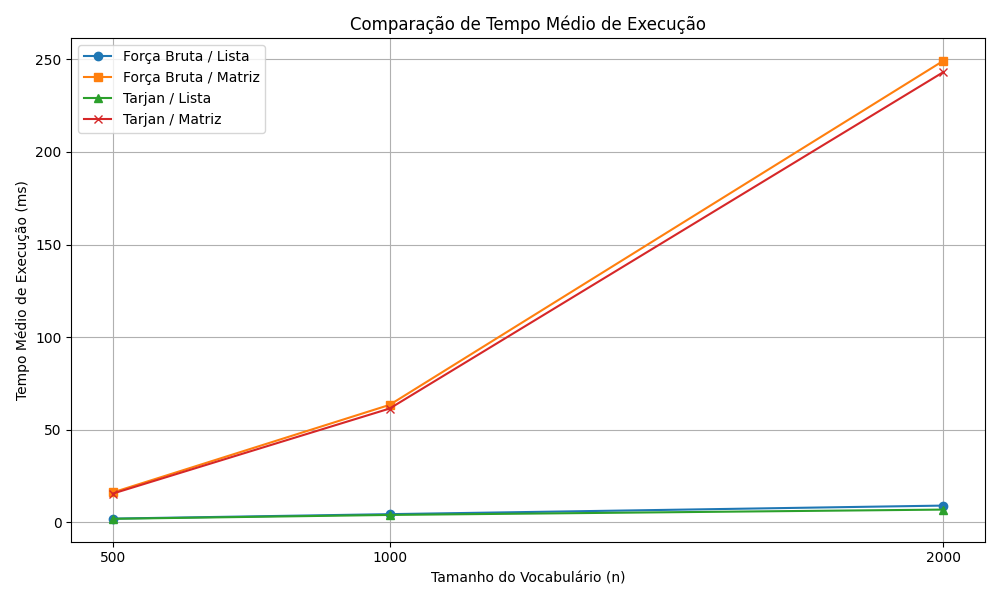
\includegraphics[width=1\textwidth]{grafico.png}
    \caption{Comparação de desempenho entre algoritmos e representações.}
\end{figure}

\section{Discussão dos Resultados}

\subsection{Desempenho dos Algoritmos de Detecção de Componentes Conexas}

\subsection*{Observações}
Compararam-se os tempos de execução médios de dois algoritmos (Força Bruta e Tarjan), utilizando duas representações distintas de grafo: \textbf{lista de adjacência} e \textbf{matriz de adjacência}.

\subsection*{Conclusões}
\begin{itemize}
    \item A principal variável de impacto no desempenho foi a \textbf{representação do grafo}, e não o algoritmo em si.
    \item A \textbf{lista de adjacência} foi significativamente mais eficiente que a matriz, principalmente em grafos grandes e esparsos — como é típico nos grafos de coocorrência.
    \item A diferença entre Força Bruta e Tarjan foi pequena dentro da mesma estrutura, com Tarjan tendo leve vantagem.
\end{itemize}

\subsection*{Implicação prática}
Para textos grandes ou aplicações que exigem performance, \textbf{usar lista de adjacência é fundamental}, independentemente do algoritmo escolhido.

\subsection{Comportamento dos Grafos em Diferentes Tipos de Texto}

\subsection*{Em textos pequenos e controlados}
\begin{itemize}
    \item Os grafos gerados tendiam a se dividir em \textbf{várias componentes conexas distintas}.
    \item Cada componente geralmente refletia um \textbf{tema ou tópico central} do texto (exemplo: palavras relacionadas a ``educação'' formando uma subestrutura separada de palavras relacionadas a ``tecnologia'').
\end{itemize}

\subsection*{Em bases textuais amplas}
\begin{itemize}
    \item O grafo passou a apresentar uma \textbf{única componente conexa gigante}, onde todas as palavras estão, de algum modo, conectadas.
\end{itemize}

\subsection*{Interpretação}
Esse fenômeno representa uma \textbf{mudança estrutural significativa} no grafo, decorrente da maior diversidade e sobreposição semântica dos textos.

\subsection{Palavras Hub e sua Influência Estrutural}

\subsection*{Definição}
Palavras \textbf{hub} são termos que ocorrem com muita frequência e aparecem em diferentes contextos. Elas funcionam como \textbf{pontes linguísticas}, conectando palavras que, de outro modo, pertenceriam a temas distintos.

\subsection*{Exemplos comuns}
\textit{``problema'', ``forma'', ``uso'', ``importante'', ``sistema'', ``realizar'', ``trabalho''}.

\subsection*{Efeitos no grafo}
\begin{itemize}
    \item Essas palavras possuem \textbf{grau elevado} e criam \textbf{conexões transversais} no grafo, unindo diferentes clusters semânticos.
    \item São as responsáveis diretas por \textbf{colapsar componentes separadas em uma só}, criando a componente conexa gigante.
\end{itemize}

\subsection{Consequências para Análise e Interpretação dos Grafos}

\subsection*{Problemas}
\begin{itemize}
    \item Dificulta a \textbf{identificação automática de tópicos} ou \textbf{comunidades temáticas}, já que tudo parece conectado.
    \item \textbf{Dilui o significado local} das coocorrências, tornando mais difícil interpretar relações semânticas específicas.
\end{itemize}

\subsection*{Estratégias para mitigar}
\begin{itemize}
    \item \textbf{Remoção de palavras hub}: além de \textit{stopwords} tradicionais, remover palavras com grau extremamente alto.
    \item \textbf{Aplicação de limiar de frequência}: manter apenas arestas com número de coocorrências acima de um certo valor.
    \item \textbf{Análise de comunidades internas}: mesmo com uma única componente, algoritmos como \textit{Louvain} podem revelar subgrupos semânticos.
    \item \textbf{Janelas menores de coocorrência}: diminuem o alcance das pontes semânticas, favorecendo agrupamentos locais.
\end{itemize}

\section{Reflexão Final}

O projeto demonstrou, na prática, como o \textbf{comportamento estrutural de um grafo de coocorrência} varia com a escala, a representação e a granularidade semântica dos dados.

Os testes controlados foram fundamentais para observar padrões e validar a teoria. Já os testes com dados reais mostraram desafios que só emergem com \textbf{complexidade e escala}.

\medskip

Em última análise, o sucesso na análise de grafos linguísticos não depende apenas do algoritmo, mas da \textbf{combinação entre representação, filtragem, escala de análise e objetivos semânticos}.


\section{Figura do Grafo com Componentes Destacados (Opcional)}

\begin{figure}[H]
    \centering
    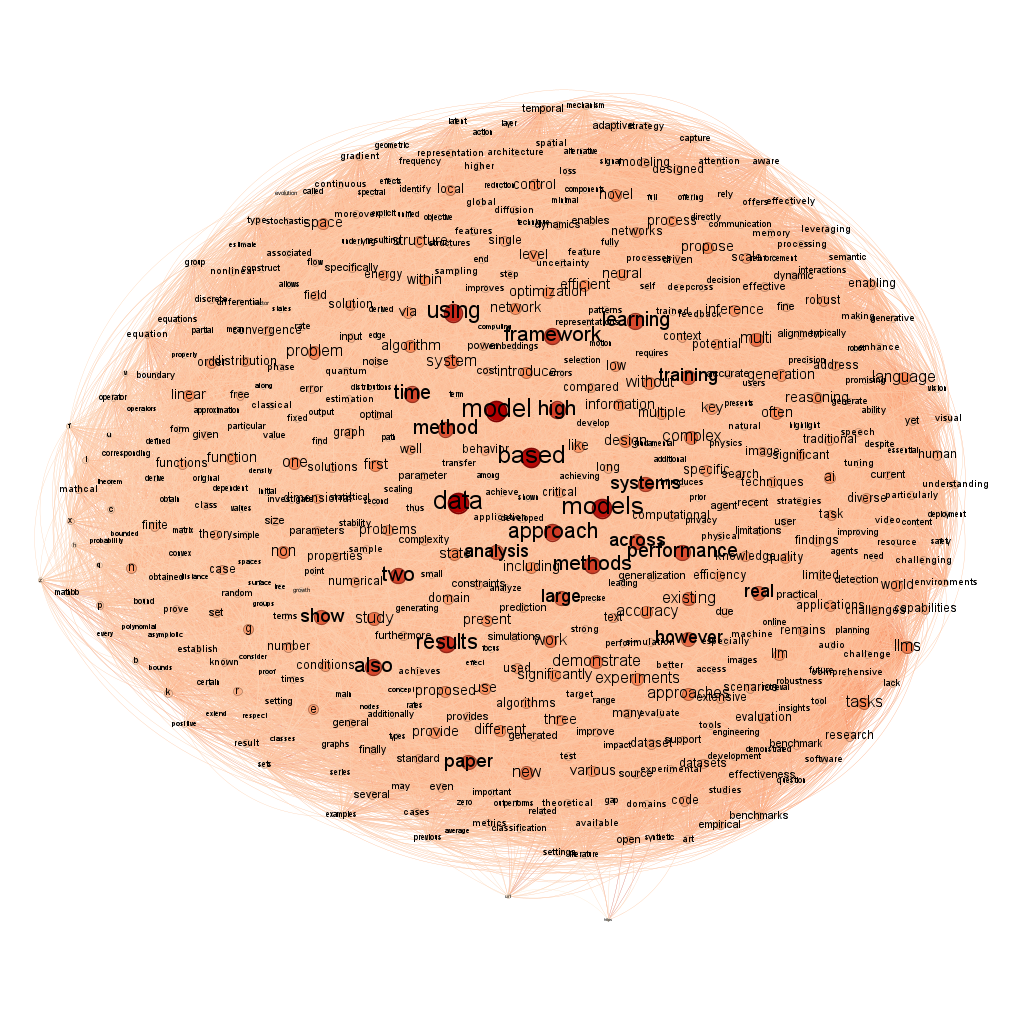
\includegraphics[width=1\textwidth]{grafo.png}
    \caption{Grafo de Coocorrência para $n = 500$ termos, gerado a partir das amostras reais mencionadas anteriormente no relatório. Cada nó representa um termo frequente, e as arestas indicam coocorrência entre termos dentro de uma janela deslizante.}
\end{figure}

\begin{figure}[H]
    \centering
    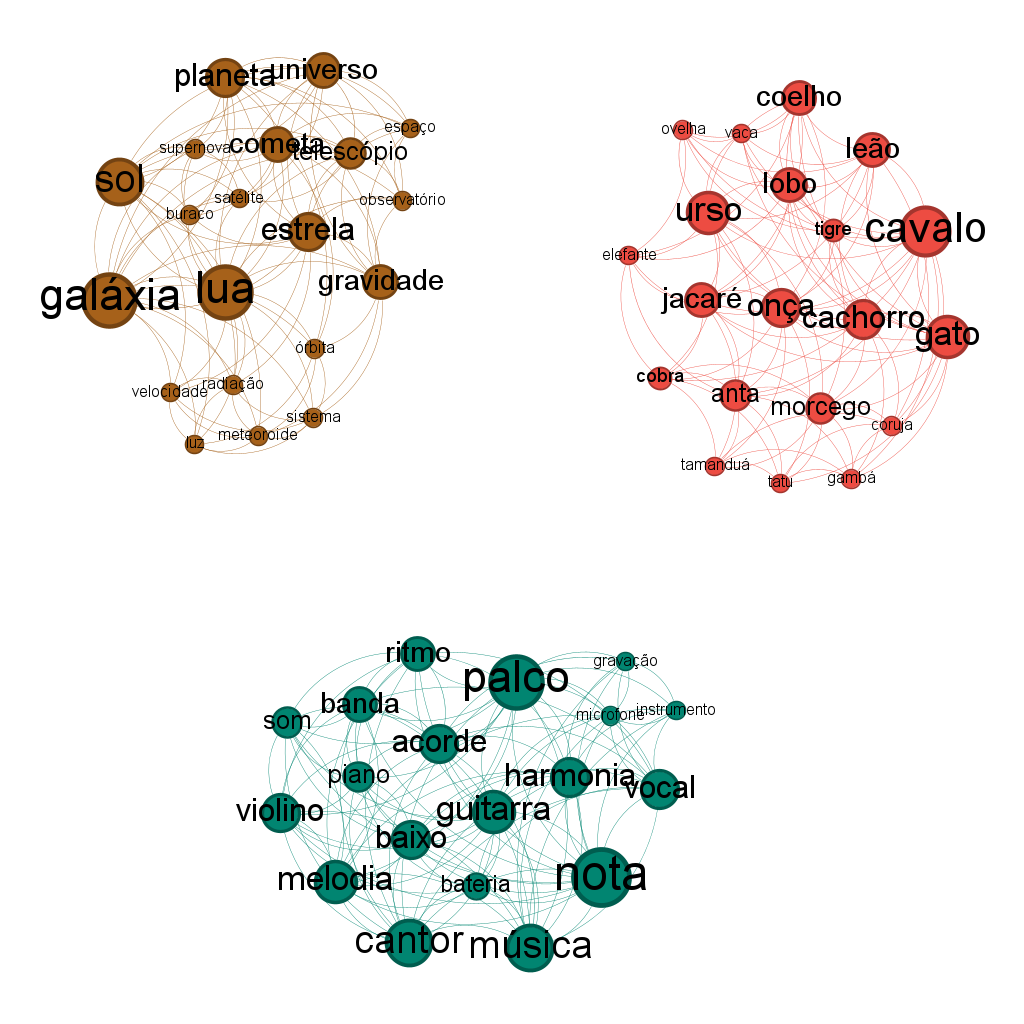
\includegraphics[width=1\textwidth]{grafoTextoTeste.png}
    \caption{Grafo de Coocorrência gerado a partir de uma base de textos sintéticos criada especificamente para testes controlados. Essa representação foi utilizada para validar o comportamento dos algoritmos de detecção de componentes conexas em diferentes cenários. Cada componete conexa está representada com uma cor diferente (como pedido no trabalho)}
\end{figure}


\end{document}
